\documentclass[11pt]{article}

\usepackage[margin=1.1in]{geometry}
\usepackage{amsmath,amssymb,amsfonts}
\usepackage{booktabs}
\usepackage{graphicx}
\usepackage{multirow}
\usepackage{microtype}
\usepackage[colorlinks=true,linkcolor=blue,citecolor=blue,urlcolor=blue]{hyperref}

\newcommand{\bx}{\mathbf{x}}
\newcommand{\bu}{\mathbf{u}}
\newcommand{\bt}{\mathbf{t}}
\newcommand{\R}{\mathbb{R}}
\newcommand{\E}{\mathbb{E}}
\newcommand{\Cin}{C_{\mathrm{in}}}
\newcommand{\Cout}{C_{\mathrm{out}}}
\newcommand{\code}[1]{\texttt{#1}}

\emergencystretch=3em

\title{Rational Basis Functions for Continuous-Kernel\\Graph Convolutions}
\author{Draft --- technical description, training recipe, and two main experiments}
\date{\today}

\begin{document}
\maketitle

\begin{abstract}
We replace the fixed B-spline basis of SplineCNN by learnable rational
(safe-Pad\'e) basis functions. Because rational functions need not be
localised, the number of basis functions $K$ --- and with it the dominant
kernel-weight parameter count $K\,\Cin\Cout$ --- decouples from the spatial
resolution $k^D$ of a spline grid. With a spline-subspace initialization and a
variance-preserving weight rescaling, $K{=}4$--$8$ non-separable rational
basis functions match or exceed $K{=}25$--$125$ B-spline hats on PascalVOC
keypoint matching (DGMC) and FAUST shape correspondence, at $2$--$5\times$
fewer parameters. All numbers are from branch
\code{worktree-spline-improve}; every table is reproduced by
\code{python benchmarks/analyze\_results.py}.
\end{abstract}

\section{Motivation}
\label{sec:motivation}

SplineCNN~\cite{fey2018splinecnn} convolves over irregular graphs with a
continuous, matrix-valued kernel expanded in a fixed B-spline basis. Because
the hat functions are \emph{localised}, covering the pseudo-coordinate domain
$[0,1]^D$ at resolution $k$ requires $K=k^D$ basis functions, each carrying
its own weight matrix: $K{=}25$ in 2-D and $K{=}125$ in 3-D for $k{=}5$. The
kernel weights $K\,\Cin\Cout$ dominate the parameter count of every SplineCNN
we study (e.g.\ 95\% of a DGMC backbone).

We replace the hats by \emph{learnable rational basis functions} (safe Pad\'e
approximants, as in PAU~\cite{molina2020pade}, rKAN~\cite{aghaei2024rkan} and
KAT~\cite{yang2025kat}, which use them as \emph{activations}; here they are
\emph{spatial kernel bases}). Rational functions are smooth, bounded by
construction, and --- crucially --- need not be localised: the number of basis
functions $K$ becomes a free capacity parameter decoupled from any spatial
resolution. Our main empirical finding is that $K{=}4$--$8$ non-localised
rational functions match or beat $K{=}25$--$125$ hats.

\section{The operator}
\label{sec:operator}

All layers compute the SplineConv form
\begin{equation}
\bx'_i \;=\; \Theta_{\mathrm{root}}\,\bx_i \;+\;
\mathop{\square}_{j\in\mathcal N(i)}\;\Bigl(\sum_{p=1}^{K} B_p(\bu_{ij})\,\Theta_p\Bigr)\bx_j \;+\; \mathbf b,
\label{eq:splineconv}
\end{equation}
with pseudo-coordinates $\bu_{ij}\in[0,1]^D$ (normalised Cartesian offsets,
\code{T.Cartesian}), weight matrices $\Theta_p\in\R^{\Cin\times\Cout}$, and
aggregation $\square \in \{\mathrm{mean}, \mathrm{add}\}$ (mean unless stated;
the FAUST reference protocol uses add, see \S\ref{sec:faust}). Only the basis
$\{B_p\}$ differs between models. Throughout, $t = 2u-1 \in [-1,1]$ and
$\phi_0,\phi_1,\dots$ are Chebyshev polynomials of the first kind
($\phi_0{=}1$, $\phi_1{=}t$, $\phi_{j+1}{=}2t\phi_j-\phi_{j-1}$;
\code{--poly monomial} is supported but slightly worse).

\paragraph{B-spline baseline} (\code{dgmc/models/bspline.py}, pure PyTorch).
$B_p$ are tensor products of degree-1 open B-splines (``hats'') on $k$
uniform knots per dimension; $2^D$ of the $K=k^D$ products are non-zero at
any $\bu$.

\paragraph{Product rational basis} (\code{RationalBasis},
\code{--rational\_basis product}).
$B_{\mathbf p}(\bu) = \prod_{d=1}^{D} r^{(d)}_{p_d}(u_d)$, a tensor product of
per-dimension learnable rational functions
\begin{equation}
r_k(u) \;=\; \frac{P_k(t)}{1+|Q_k(t)|}, \qquad
P_k(t)=\sum_{j=0}^{m} a_{k,j}\,\phi_j(t), \quad
Q_k(t)=\sum_{j=1}^{n} b_{k,j}\,\phi_j(t),
\label{eq:safepade}
\end{equation}
with degrees $(m,n)=(5,4)$ (\code{--degrees 5 4}). This is the \emph{safe}
Pad\'e form, variant~B; variant~A uses $1+\sum_j |b_{k,j}\phi_j(t)|$
(\code{--safe A}, slightly worse). The denominator is $\ge 1$, so no pole can
form. Indexing matches the hat basis (first dimension fastest), so the
$\Theta_p$ are shape-compatible with SplineConv. Still $K=\prod_d k_d$
functions.

\paragraph{Multivariate rational basis.} Each basis function is a single
\emph{non-separable} rational function of all coordinates
(\code{MultivariateRationalBasis}, \code{--rational\_basis multivariate}),
\begin{equation}
B_p(\bu) = \frac{P_p(\bt)}{1+|Q_p(\bt)|},\qquad
P_p(\bt)=\!\!\sum_{|\alpha|\le m}\! a_{p,\alpha}\prod_d \phi_{\alpha_d}(t_d),\quad
Q_p(\bt)=\!\!\sum_{1\le|\alpha|\le n}\! b_{p,\alpha}\prod_d \phi_{\alpha_d}(t_d),
\label{eq:multivariate}
\end{equation}
with multi-indices $\alpha\in\mathbb N_0^D$ of \emph{total degree}
$|\alpha|\le m$ (numerator, $\binom{m+D}{D}$ terms) and $|\alpha|\le n$
(denominator, $\binom{n+D}{D}{-}1$ terms, no constant). We use $(m,n)=(8,6)$
--- a product of two degree-5 polynomials has total degree 10, so $(5,4)$
underfits the hat targets (fit RMSE $3\times$ worse) and yields no gain over
SplineCNN. \textbf{$K$ is free} (\code{--num\_bases $K$}), independent of any
grid. Coefficient counts are negligible: at $D{=}2$, $(8,6)$ has $45{+}27=72$
scalars per basis function.

\paragraph{MLP control} (\code{MLPBasis}, \code{--rational\_basis mlp}).
$\bu \mapsto \mathrm{Lin}_K(\mathrm{ReLU}(\mathrm{Lin}_{64}(\bt)))$ --- the
filter-generating network of SchNet/PointConv with the same $\Theta_p$, used
to attribute gains to the rational \emph{form} rather than to ``any learned
$K$-dimensional basis''.

\paragraph{Cost.} Parameters: $K\,\Cin\Cout + \Cin\Cout + \Cout$ per layer
plus the basis coefficients. Compute: rational bases evaluate all $K$
functions densely per edge (no sparsity), costing ${\sim}12$--$40\%$ more
time per epoch than the pure-PyTorch spline at equal $K$ in 2-D and
${\sim}2\times$ at large feature counts; decreasing $K$ recovers most of it.

\section{Initialization}
\label{sec:init}

Initialization is the single most important design choice; a bad one costs
0.7--90 accuracy points (\S\ref{sec:secondary}).

\paragraph{Spline (hat) fit --- default for grid-$K$.} Fit each rational
function to its B-spline hat by least squares so the layer \emph{starts as a
SplineConv}: closed-form LS fit of the numerator with $Q\equiv 0$, then joint
refinement of $(a,b)$ with Adam (lr $0.02$, 500 steps) followed by L-BFGS
(100 iterations, strong-Wolfe line search), in float64, on a fixed grid (1-D:
256/1024 points; 2-D: $32^2$; 3-D: $16^3$). Two essential details:
\begin{enumerate}
\item \textbf{Never start the denominator at exactly zero.}
  $\partial|Q|/\partial b = \mathrm{sign}(Q)\,\phi_j$ vanishes identically at
  $b=0$ ($\mathrm{sign}(0)=0$), freezing the denominator forever --- the
  model silently degrades to a polynomial basis. We start
  $b \sim \mathcal N(0, 0.01^2)$.
\item The fit is cached per configuration within a process, so stacked layers
  share one fit (${\sim}20$\,s in 3-D instead of ${\sim}45$\,min for a
  6-layer model).
\end{enumerate}

\paragraph{PCA-of-hats --- for free $K$.} When $K \ne k^D$, fit the $K$
functions to the $K$ leading principal components (left singular vectors,
deterministic sign, rescaled to unit max) of the $k^D$ hat basis evaluated on
the grid: the $K$-dimensional subspace that best approximates the SplineConv
kernel space. $K=k^D$ recovers the hats exactly. Caveat: components come in
degenerate symmetric pairs, and the higher components are oscillatory --- at
$K\ge 16$ in 3-D this init is seed-fragile (\S\ref{sec:faust}).

\paragraph{Variance-preserving (vp) gain} (adapted from
KAT~\cite{yang2025kat}). After basis init, scale the kernel weights by
$\sqrt{\alpha}$ with
\begin{equation}
\alpha \;=\;
\E_{\bu}\Bigl[\sum_p \mathrm{hat}_p(\bu)^2\Bigr] \Big/\;
\E_{\bu}\Bigl[\sum_p B_p(\bu)^2\Bigr]
\label{eq:vp}
\end{equation}
(numerical integration on a grid), so any init produces messages at
SplineConv scale. $\alpha \approx 1.00$ for hat-fitted bases (a no-op),
$0.57$ for Gaussian-fitted, $0.06$--$0.14$ for raw-Chebyshev, $0.018$ for
constant-one. It rescues mis-scaled inits (raw-Chebyshev on WILLOW:
$46\% \to 97\%$) but never substitutes for a good target shape.

\paragraph{What fails, and why (ablation summary).} Ranking over PascalPF~/
WILLOW~/ PascalVOC: hat-fit $\gtrsim$ Gaussian-bump fit $\gg$ raw Chebyshev
($+$vp) $\gg$ random ($B_p\!\approx\!1/K$; $-0.7$ to $-5.8$ pts) $\gg$
constant-one ($B_p\!\equiv\!1$, catastrophic). The constant init fails for
two reasons: (i)~without vp its output scale is $\sqrt{K}$-fold too large and
the DGMC softmax saturates (gradients $\to 0$); (ii)~\emph{with} vp it still
fails, because all $K$ identical basis functions give all $\Theta_p$
identical gradients, and Adam's per-parameter normalisation then moves
$\sum_p\Theta_p$ $K\times$ faster than the learning rate suggests ---
verified: training survives at $\mathrm{lr}/K$ but not at $\mathrm{lr}/5$.
Weight decay on basis coefficients only (\code{--basis\_wd}) had no
measurable effect ($-0.26$, n.s.).

\section{Training details (common)}
\label{sec:training}

Adam (PyTorch defaults, $\beta=(0.9,0.999)$), no weight decay. The basis
coefficients are trained jointly with everything else at the same learning
rate. Kernel weights use SplineConv's uniform init with bound
$1/\sqrt{K\,\Cin}$ (matching PyG's root/bias init instead --- bound
$1/\sqrt{\Cin}$, zero bias --- was tested and changes nothing: 97.31 vs
97.23 on FAUST). All experiments log to wandb (losses split into the
$S^{(0)}$/$S^{(L)}$ terms where applicable, train/test accuracy, per-step
gradient norm, update norm $\|\Delta\theta\|$, parameter norm, timings).

\section{Experiment 1 --- PascalVOC keypoint matching (DGMC)}
\label{sec:pascalvoc}

\paragraph{Setup} (\code{examples/pascal.py}, defaults unless noted).
DGMC~\cite{fey2020dgmc} on PascalVOC-Keypoints with Berkeley annotations:
graphs from \code{T.Delaunay + FaceToEdge} (tolerant variant:
$<3$-keypoint graphs have no faces), node features = frozen VGG16-bn
relu4\_2\,$\|$\,relu5\_1 (1024-d), pseudo-coordinates 2-D anisotropic
\code{T.Cartesian} ($D{=}2$). Backbones $\psi_1$ ($1024\to256$, cat=False,
dropout 0.5) and $\psi_2$ ($128\to128$, cat=True, dropout 0), both 2 conv
layers; $L{=}10$ consensus steps. Adam lr $10^{-3}$, batch 512 graph pairs,
\textbf{15 epochs}, self-supervised pairs (\code{ValidPairDataset}), test:
1000 samples/category, metric = mean over the 20 categories of
keypoint-matching accuracy at the final epoch; \textbf{5 seeds} (0--4).
Rational configs: multivariate, $(m,n)=(8,6)$, safe~B, Chebyshev; PCA init
$+$ vp for free-$K$; hat-fit init for $K=k^D$ (``mv $k{=}3$'' =
kernel\_size~3, $K{=}9$).

\begin{table}[ht]
\centering
\footnotesize
\setlength{\tabcolsep}{4pt}
\begin{tabular}{lrrll}
\toprule
config & $K$ & params & final acc & best acc \\
\midrule
SplineCNN $k{=}5$ & 25 & 9.50M & $72.00 \pm 0.39$ & $73.00 \pm 0.40$ \\
SplineCNN $k{=}3$ & 9 & 3.74M & $72.06 \pm 0.85$ & $72.78 \pm 0.40$ \\
SplineCNN $k{=}2$ & 4 & 1.93M & $70.94 \pm 0.63$ & $71.48 \pm 0.40$ \\
product rational $k{=}5$ & 25 & 9.50M & $72.24 \pm 0.67$ & $72.88 \pm 0.48$ \\
product rational $k{=}3$ & 9 & 3.74M & $72.62 \pm 0.41$ & $73.26 \pm 0.18$ \\
\textbf{multivariate, hat init, $k{=}3$} & 9 & 3.74M & $\mathbf{73.76 \pm 0.81}$ & $\mathbf{74.12 \pm 0.48}$ \\
multivariate, PCA$+$vp, $K{=}4$ & 4 & 1.94M & $72.92 \pm 0.36$ & $73.78 \pm 0.41$ \\
multivariate, PCA$+$vp, $K{=}6$ & 6 & 2.66M & $73.10 \pm 0.41$ & $74.06 \pm 0.37$ \\
multivariate, PCA$+$vp, $K{=}9$ & 9 & 3.74M & $73.16 \pm 0.47$ & $73.72 \pm 0.19$ \\
multivariate, PCA$+$vp, $K{=}16$ & 16 & 6.26M & $72.26 \pm 0.42$ & $73.26 \pm 0.42$ \\
multivariate, PCA$+$vp, $K{=}2$ / $K{=}1$ & 2 / 1 & 1.21M / 0.85M & 71.44 / 67.98 & \\
MLP basis, $K{=}4$ / $K{=}9$ & 4 / 9 & 1.94M / 3.74M & $72.12 \pm 0.32$ / $71.46 \pm 0.64$ & \\
multivariate $(5,4)$, $k{=}5$ (degree control) & 25 & 9.51M & $72.04 \pm 0.94$ & \\
\bottomrule
\end{tabular}
\caption{PascalVOC keypoint matching (DGMC), mean $\pm$ std over 5 seeds.}
\label{tab:pascalvoc}
\end{table}

\begin{figure}[ht]
\centering
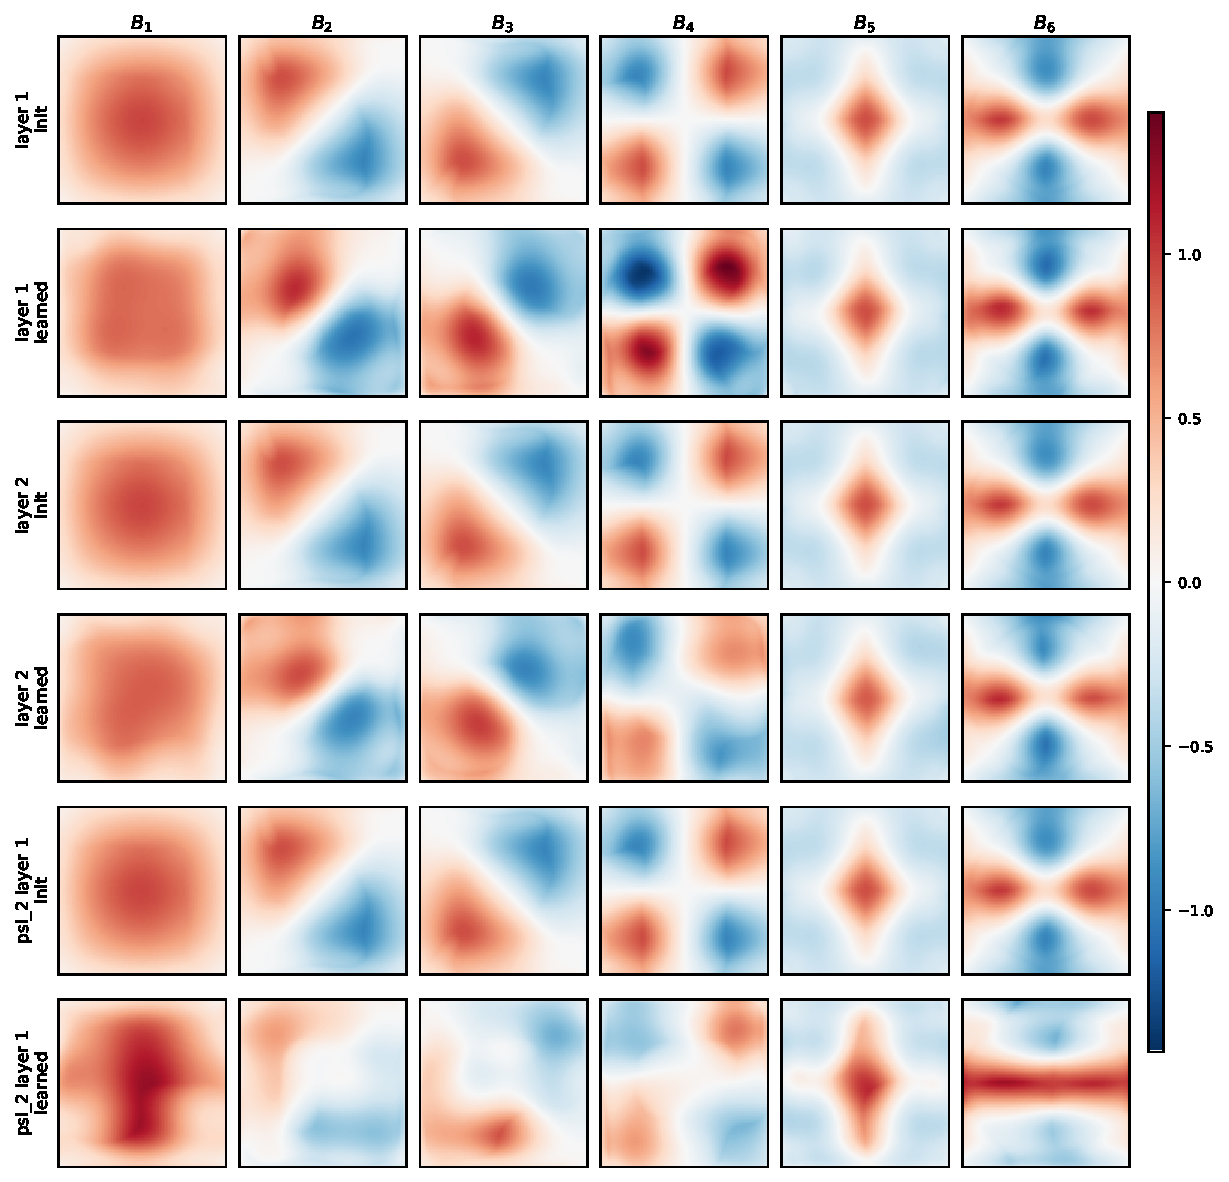
\includegraphics[width=\linewidth]{figures/basis_voc_mv_K6.pdf}
\caption{Learned multivariate rational basis functions of the PascalVOC
model \code{mv\_K6} ($K=6$, degrees $(8,6)$, PCA-of-hats initialization,
seed 0) on the pseudo-coordinate square $[0,1]^2$ (Cartesian edge attributes,
$(0.5,0.5)$ = zero offset). Rows alternate between the initialization
(the six leading principal components of the $5\times 5$ B-spline hats) and
the functions after 15 epochs, for both layers of $\psi_1$ and the first
layer of $\psi_2$. The learned functions keep the overall layout of their
initialization but sharpen and shift their extrema and develop asymmetric
side lobes; the $\psi_2$ layer, which operates on the consensus features,
moves furthest from its initialization. Figures for the hat-initialized
$K=9$ basis and for $K=4$ are in \code{paper/figures/}
(\code{experiments/plot\_basis.py}).}
\label{fig:basis_voc}
\end{figure}


Welch t-tests: mv-hat $k{=}3$ vs SplineCNN $k{=}5$: $+1.76$, $p=0.005$; vs
product $k{=}3$: $+1.14$, $p=0.032$. $K{=}4$ vs SplineCNN $k{=}5$: $+0.92$,
$p=0.005$; vs MLP $K{=}4$: $+0.80$, $p=0.006$; vs SplineCNN $k{=}2$ (equal
$K$ and params): $+1.98$, $p=0.001$. The accuracy--$K$ curve is flat for
$K\in[4,9]$ and \emph{drops} at $K{=}16$ (overfitting); the $(5,4)$ control
shows the total degree matters.

\section{Experiment 2 --- FAUST shape correspondence}
\label{sec:faust}

\paragraph{Setup} (\code{examples/faust.py}, mirroring the SplineCNN
paper~/ PyG example). 100 registered human meshes (6890 vertices, 13776
faces), 80 train~/ 20 test; task: classify every vertex of a test mesh into
one of 6890 template-vertex classes; metric: exact-match accuracy. Input
\code{T.Constant(1)}; pseudo-coordinates 3-D \code{T.Cartesian} ($D{=}3$).
Network: 6 conv layers ($1\to32\to64\times5$), ELU, then Lin(64,\,256), ELU,
dropout 0.5, Lin(256,\,6890), log-softmax; NLL loss. Adam lr
$0.01 \to 0.001$ at epoch 61, batch 1, \textbf{100 epochs},
\textbf{gradient-norm clipping 1.0} (all backbones --- see below),
aggregation \code{add} (the PyG reference) unless ``mean''; \textbf{3
seeds}. Rational configs: multivariate $(8,6)$, PCA init $+$ vp,
\code{--num\_bases $K$}; product $k{=}3$ with hat init.

\begin{table}[ht]
\centering
\footnotesize
\setlength{\tabcolsep}{4pt}
\begin{tabular}{lrrl}
\toprule
config & $K$ & params & final acc \\
\midrule
\textbf{multivariate $K{=}8$} & 8 & 1.97M & $\mathbf{99.41 \pm 0.04}$ \\
\textbf{multivariate $K{=}4$} & 4 & 1.89M & $\mathbf{99.38 \pm 0.09}$ \\
product rational $k{=}3$ & 27 & 2.30M & $99.24 \pm 0.08$ \\
\emph{SplineCNN paper (CUDA kernel)} & 125 & 4.1M & \emph{99.20} \\
multivariate $K{=}4$, mean aggr & 4 & 1.89M & $98.93 \pm 0.10$ \\
SplineCNN $k{=}5$, mean $+$ clip (best reproduction) & 125 & 4.11M & $98.71 \pm 0.08$ \\
MLP basis $K{=}8$ & 8 & 1.96M & $98.21 \pm 1.11$ \\
SplineCNN $k{=}5$, add $+$ clip & 125 & 4.11M & $97.23 \pm 0.51$ \\
SplineCNN $k{=}3$ & 27 & 2.30M & $83.6 \pm 15.6$ \\
multivariate $K{=}16$ / $K{=}27$ & 16 / 27 & 2.13M / 2.34M & $70.4 \pm 25.2$ / $19.0 \pm 32.8$ \\
SplineCNN $k{=}5$, add, no clip (literal PyG example) & 125 & 4.11M & $29.1 \pm 50.3$ \\
SplineCNN $k{=}2$ & 8 & 1.95M & $3.4 \pm 3.3$ \\
\bottomrule
\end{tabular}
\caption{FAUST shape correspondence, mean $\pm$ std over 3 seeds.}
\label{tab:faust}
\end{table}

\paragraph{Notes.} (i)~\emph{Reproduction gap and stability}: the PyG
example's \code{aggr='add'} deviates from the paper's degree-normalised
operator; with mesh degree $\approx 6$ it destabilises training (2/3 seeds
collapse to uniform output after a gradient spike) and costs $\approx 1.5$
pts even when rescued by clipping. With mean aggregation $+$ clipping,
SplineCNN reproduces to within 0.5 pts of the paper. Clipping is required
under either aggregation (mean/no-clip: $96.9 \pm 1.7$).
(ii)~\emph{Small $K$}: SplineCNN cannot be made small in 3-D ($K{=}27$ loses
a seed, $K{=}8$ fails entirely), whereas $K{=}4$--$8$ rational functions
exceed the published SplineCNN number at $2.2\times$ fewer parameters and
the lowest variance in the table --- under the \emph{harder} add protocol.
(iii)~\emph{Large-$K$ fragility}: with PCA init, $K\ge16$ in 3-D is
seed-fragile (slow or collapsed in 2/3 seeds) --- an init problem
(oscillatory components, small vp gain), not a capacity limit. (iv)~The MLP
control shows non-localisation alone helps, but the rational form adds
$+1.2$ pts and $25\times$ lower variance.

\section{Secondary experiments (summary)}
\label{sec:secondary}

\paragraph{WILLOW-ObjectClass} (DGMC, no VOC pretraining, 10 runs $\times$
15 epochs, 20 train images/class): spline $96.80 \pm 1.20$, product rational
$97.28 \pm 1.01$, multivariate $k{=}5$ $97.55 \pm 0.63$ (all n.s.; duck
dominates variance). Per-epoch curves: all bases memorise the 380 train
pairs/class by epoch ${\sim}8$; test accuracy saturates without decay, test
loss drifts up mildly (over-confidence). Init ablation (product basis):
Gaussian-fit 97.72 (best), hat-fit 97.28, cheb$+$vp 97.07, random$+$vp
92.13, constant (any variant) 10.00 $=$ chance.

\paragraph{PascalPF} (synthetic $+$ PascalPF pairs, 3 seeds $\times$ 20
epochs): rational $k{=}3$ $95.73 \pm 0.06$ $>$ spline $k{=}5$
$95.27 \pm 0.15$; Gaussian-fit init 95.90; random init 94.93; constant init
78/66. On PascalVOC the same init ordering holds but reversed between gauss
and hat: hat-fit 73.76 $>$ gauss 72.40 ($p=0.018$) $>$ cheb$+$vp 71.62.

\section{Practical recipe}
\label{sec:recipe}

\begin{enumerate}
\item Use the multivariate basis, total degrees $(8,6)$, safe-B, Chebyshev.
\item Choose $K \approx 4$--$8$, independent of dimension.
\item Init: hat-fit when $K=k^D$, else PCA-of-hats; always with the vp gain;
  never a zero denominator.
\item Train exactly like the SplineCNN you are replacing; add grad-norm
  clipping for deep stacks with add-aggregation.
\item Expect $\approx$ equal accuracy at ${\sim}2$--$5\times$ fewer
  parameters, or $+0.7$--$1.8$ pts at equal parameter count; expect
  10--40\% slower epochs.
\end{enumerate}

\section{Open questions / limitations}
\label{sec:limitations}

\begin{itemize}
\item Large-$K$ PCA-init fragility in 3-D (localised targets for the higher
  components should fix it).
\item Basis-coefficient scale drift at large $K$ (safe-Pad\'e gauge freedom;
  benign on accuracy, visible in parameter norms~/ calibration).
\item Mean vs add aggregation interacts with the basis (mean helps spline,
  mildly hurts rational on FAUST); unexplained.
\item Timing uses a pure-PyTorch SplineConv baseline; against the CUDA
  \code{torch-spline-conv} kernel the rational overhead would be larger.
\item WILLOW/PascalPF gains are within seed noise; the significant results
  are PascalVOC and FAUST.
\end{itemize}

\begin{thebibliography}{9}

\bibitem{fey2018splinecnn}
M.~Fey, J.~E. Lenssen, F.~Weichert, and H.~M\"uller.
\newblock SplineCNN: Fast geometric deep learning with continuous B-spline
  kernels.
\newblock In \emph{CVPR}, 2018.

\bibitem{fey2020dgmc}
M.~Fey, J.~E. Lenssen, C.~Morris, J.~Masci, and N.~M. Kriege.
\newblock Deep graph matching consensus.
\newblock In \emph{ICLR}, 2020.

\bibitem{molina2020pade}
A.~Molina, P.~Schramowski, and K.~Kersting.
\newblock Pad\'e activation units: End-to-end learning of flexible activation
  functions in deep networks.
\newblock In \emph{ICLR}, 2020.

\bibitem{aghaei2024rkan}
A.~A. Aghaei.
\newblock rKAN: Rational Kolmogorov--Arnold networks.
\newblock \emph{arXiv:2406.14495}, 2024.

\bibitem{yang2025kat}
X.~Yang and X.~Wang.
\newblock Kolmogorov--Arnold transformer.
\newblock In \emph{ICLR}, 2025.

\end{thebibliography}

\end{document}
